\section{Case Study}\label{sec:eval}

In this section, we evaluate Osazone by an example, with eight language implemented.
We aim to show how the language is progressively extended and specialized by translation rules.
The languages discussed in this section and their relation are shown in the Fig. \ref{fig:langs},
 where horizontal arrows represent meta-extensions and monad extensions,
 and vertical arrows stand for specification by translation rules.

\begin{figure}
  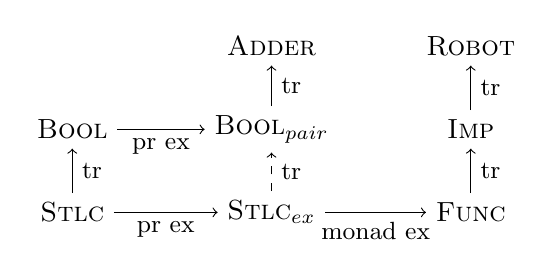
\begin{tikzpicture}[x=6pt,y=3pt,yscale=1,xscale=1]
%uncomment if require: \path (0,300); %set diagram left start at 0, and has height of 300

\node (STLC) at (-2,10) {\textsc{Stlc} };
\node (Bool) at (-2,20) {\textsc{Bool} };
\node (Boolp) at (10,20) {\textsc{Bool}$_\text{pair}$};
\node (Adder) at (10,30) {\textsc{Adder} };
\node (STLCex) at (10,10) {\textsc{Stlc}$_\text{ex}$};
\node (Ref) at (22,10) {\textsc{Func} };
\node (Imp) at (22,20) {\textsc{Imp} };
\node (Robot) at (22,30) {\textsc{Robot} };

\draw[->] (STLC) -> node[right] {\small tr} (Bool); 
\draw[->] (Bool) -> node[below] {\small pr ex} (Boolp);
\draw[->] (STLC) -> node[below] {\small pr ex} (STLCex);
% \draw[->] (STLC) -- node[below] {\small pr ex} (STLC-|STLCex) 
%  -> node[right] {\small tr} (STLCex);
\draw[->] (STLCex) -> node[below] {\small monad ex} (Ref); 
%\draw[->] (Ref) -> node[below] {\small monad ex (IO)} (RefIo);
\draw[->] (Ref) -> node[right] {\small tr} (Imp); 
\draw[->] (Imp) -> node[right] {\small tr} (Robot); 
\draw[->] (Boolp) -> node[right] {\small tr} (Adder); 
\draw[->, dashed] (STLCex) -> node[right] {\small tr} (Boolp); 
\end{tikzpicture}

  \caption{Languages for Examples}
  \label{fig:langs}
\end{figure}

%  implementing some languages based on \STLC. 
Some of these language have been discussed.
We start with \STLC, a language with lambda calculus and Boolean values.
From \STLC, we define \textsc{Bool} using translation rules.
By extending \textsc{Bool} with meta-extensions, we get $\textsc{Bool}_{\text{pair}}$ supporting pairs and projection.
With two additional translation rules, we implement a DSL \textsc{Adder} that can simulate half adders and full adders.

From another dimension, we start with meta-extensions on \STLC.
Language constructs pairs, sums, fixpoints and lists,
 introduced in Chapter 11 of Types and Programming Languages\cite{tapl} are tested.
And let bindings and ascription are implemented by translation rules.
We name the new language as \STLCex.
% In this language, we will talk about the impact of fixpoints on abstraction.

Then, we introduce reference and I/O by monad extension, getting \textsc{Ref}.
Taking \textsc{Ref} as the host language,
 we implement an imperative language \textsc{Imp}.
% The point we should care about in \textsc{Imp} is that,
%  recursive translation rules are declared in $\<while>$.
% As an extension of our framework,
%  we will discuss weak-abstraction semantics derivation.
%
% After that, we make \textsc{Ref} support I/O, getting \RefIO.
Based on \textsc{Imp}, we implement a DSL named \textsc{Robot}.
The language assumes that a robot is located at some starting coordinates,
 and users can control its movement, or print out its position with commands.
In this example, We will talk about how to access ``global variables'' in the translation rules.

\subsection{\STLCex: Fixpoint}\label{sec:fix}

Fixpoint is a common approach to implement recursion in functional programming language.
As a primitive language construct, the evaluation rule and typing rule of $\<fix>$ are specified:
\begin{align*}
  \ctr{Fix}{ \<fix>~e} & \cqq \Let{λx:t.e_1}{\EE{e}} \EE{e_1[\<fix>~(λx:t.e_1)/x]}
  % \TT{\<fix>~e} & \cqq \TT{e}:(t_1->t_2\mid t_1=t_2 |> t_1). 
\end{align*}

Since an expression with substituion are evaluated,
 the evaluation rule is not structural.
And as mentioned above, nonstructural evaluation rule should be considered how to maintain abstraction.

In fact, thanks to lambda exposure and the existing discussion on substitution, fixpoint is easy to solve.
However, unfolding according to the rules of $\<fix>$ leads to non-termination of the algorithm.
We assume that fix can be preserved in the DSL--for a language that contains recursion is straightforward.
We add the following rule to the $\dd$:
\[ \dd(\HH{\<fix>~\mexp}) = \Let{λx\!:\!t.e_1}{\dd(\HH{\mexp})} \HH{\<fix>~(λx:t.e_1)} \]
where we do not expand the substitution with fixpoint resursively.
The above rule is equivalent to the extended rule in Section \ref{sec:alg-ex}, but the $\<fix>$ is kept in the rules for readability.

\begin{example}
\[ \<iseven> => \<fix>~(λie\!:\!int->bool.~λx\!:\!int.~\<if>~(x=lit~0)~\<true>~(\<if>~(x=lit~1)~\<false>~(ie~(x-lit~2)))) \]
  
The first step is lambda exposure. The following translation rules are generated.
\begin{align*}
  \<iseven>'~e_1~e_2 & => \<if>~(e_2=lit~0)~\<true>~(\<if>~(e_2=lit~1)~\<false>~(e_1~(e_2-lit~2))) \\
  \<iseven> & => \<fix>~(λie\!:\!int->bool.~λx\!:\!int.~\<iseven>'~ie~x)
\end{align*}

The evaluation rules of language constructs used by $\<iseven>'$ all have structural semantics.
So the evaluation rule of $\<iseven>'$ is also structural.
The evaluation rule of $\<iseven>$ can be derived by:
\begin{align*}
  & \ctr{IsEven}{\<iseven>} \\
  \cqq~ & \dhl{\HH{\<fix>~(λie\!:\!int->bool.~λx\!:\!int.~\<iseven>'~ie~x)}} \\
  =~ & \Let{λx'\!:\!t.e}{\dhl{\HH{λie\!:\!int->bool.~λx\!:\!int.~\<iseven>'~ie~x}}} \HH{\<fix>~(λx':t.e)} \\
  =~ & \HH{\<fix>~(λie\!:\!int->bool.~λx\!:\!int.~\<iseven>'~ie~x)}
\end{align*}
Because of lambda exposure, $\<iseven>'$ is a DSL construct. The abstraction property holds.
\end{example}



\subsection{\textsc{Imp}: Recursive Translation Rules}\label{sec:while}

Our \textsc{Imp} language is defined by translation rules based on \textsc{Ref},
 which means the use of variables should be reference-based.
Therefore, the syntax of \textsc{Imp} here is slightly different from the general language.
First, the declarations and initial values of variables are necessary.
For example, a legal \textsc{Imp} program is
\[ \<let>~x=\<ref>~1~\<in>~x:=!x+1; !x \]
And $x:=1;x:=x+1;x$ is not permitted for $x$ not in scope.
Also, we find that what is assigned in the declaration must be a reference to some expression.
In order to simulate the syntax of declaration in common imperative language,
 we can define syntactic sugar $\<var>$ shown in Fig. \ref{fig:imp}.
The semicolon is used as part of the syntax of the declaration, to ensure that $x$ is valid in $e_2$.

Second, in \textsc{Imp}, the left-hand side of an assignment must be a variable
 and the any variable at right-hand side refers to the value stored in it (a location).
Regretfully, we are not able to simplify this by translation rules,
 and explicit dereferences are essential.
A solution is to distinguish such $x$ by the parser, and transform to $!x$ in abstract syntax tree automatically.
We still write dereferences in the following discussion.

\begin{figure}
  \begin{align*}
    \<var>~x=e_1; e_2 & => \<let>~x=\<ref>~e_1~\<in>~e_2 \\
    \<when>~e_1~e_2 & => \<if>~e_1~e_2~() \\
    e_1 +\!\! = e_2 & => e_1 := !e_1 + e_2 \\
    \<while>~e_1~\<do>~e_2~\<end> & => \<if>~e_1~(e_2; \<while>~e_1~\<do>~e_2~\<end>)~()
  \end{align*}
  \caption{Translation Rules for \textsc{Imp}}
  \label{fig:imp}
\end{figure}

Some other common language constructs in \textsc{Imp} are defined in Fig. \ref{fig:imp}.
But $\<while>$, whose definition does not satisfy requirement \ref{req:no-recursion}, is our concern.
By the algorithm extension of Section \ref{sec:alg-ex}, we have
\begin{align*}
  & \ctr{While}{\<while>~e_1~\<do>~e_2~\<end>} \\ 
  \cqq~~ & \dhl{\EE{\<if>~e_1~(e_2; \<while>~e_1~\<do>~e_2~\<end>)~()}} \\
  =~~ & \EE{e_1}:\branch{
        \<true> |> \Let{()}{\EE{e_2}} \dhl{\EE{\<while>~e_1~\<do>~e_2~\<end>}} \\&
        \<false> |> ()
    } \\
  =~~ & \EE{e_1}:\branch{
      \<true> |> \Let{()}{\EE{e_2}} \EE{\<while>~e_1~\<do>~e_2~\<end>} \\&
      \<false> |> ()
  }
\end{align*}
% Consider that we discard this step of expansion, the evaluation rule of $\<while>$ can be derived as follows, 
%  which is not structural but correct:
% \[ 
%   \ctr{While}{\<while>~e_1~\<do>~e_2~\<end>} \cqq \EE{e_1}:\branch{
%     \<true> |> \Let{()}{\EE{e_2}} \EE{\<while>~e_1~\<do>~e_2~\<end>} \\&
%     \<false> |> ()
%   } 
% \]
Because $\<while>$ itself is a language construct in the DSL,
 we can think of it as satisfying abstraction if we keep it in the evaluation rule.

% The more serious problem is the type derivation.
% It is reasonable that $\<while>$ has a recursive evaluation,
%  but the typing of $\<while>$ should not be.
% If the above approach is applied, an error typing rule is generated:
% \begin{align*}
%   \TT{\<while>~e_1~\<do>~e_2~\<end>} \cqq~
%   & \Let{\<bool>}{\TT{e_1}} \Let{\<unit>}{\TT{e_2}} \\
%   & \Let{t_2}{\TT{\<while>~e_1~\<do>~e_2~\<end>}} \<unit>:(t_3 \mid t_2=t_3 |> t_2)
% \end{align*}
% In this instance, the typing rule must be specified manually.

More problem arise when \textsc{Imp} is used as a host language.
When a language construct is translated to $\<while>$,
 abstraction is difficult to guarantee.
For example, $\<for>$ can be defined as follows, but we cannot derive an evaluation rule without $\<while>$.
\[ \<for>~(e_1;e_2;e_3)~\<do>~e_4 => e_1;\<while>~e_2~\<do>~(e_4;e_3)~\<end> \]



\subsection{\textsc{Robot}: Access to Global Variables}

The goal of this language is to achieve simple control of robots in a two-dimensional plane.
A sample program of \text{Robot} is:
\[ \mathit{robot~5~5~\{ up, up, right, whereAmI, left, whereAmI \}} \]
where $\mathit{robot}~5~5\{...\}$ declares a robot with a starting point of $(5,5)$,
and the braces contain a series of commands to be executed on the robot, splitted by comma.
Some commands are used to control the movement of the robot,
 and command $\mathit{whereAmI}$ will print current position.

As a natural idea, we record the current position of the robot via the global variables $x$ and $y$.
Then each command reads and manipulates global variables,
 and comma is defined as sequencing.
These language constructs are defined as follows:
\begin{align*}
  \<robot>~e_1~e_2~\{e\} & => \<let>~x=\<ref>~e_1,y=\<ref>~e_2~\<in>~e \\
  e_1,e_2 & => e_1;e_2 \\
  \<left> & => x:=\ !x-1 \\
  \<whereAmI> & => \<print>~!x; \<print>~!y
\end{align*}
where $x$ and $y$ are literal identifiers.
But requirement \ref{req:close} is not satisfied.
Since variables without local bindings cannot be used directly in translation rules,
 it is necessary to pass the value of the variable as an argument to the language constructs or as an argument to a lambda abstraction.
Hence, $\<left>$ can be expressed as
\[ \<left> => λpos:(\<Rf>~\<int>)\times (\<Rf>~\<int>). ~(\<fst>~pos)~ \texttt{-=}~ 1; pos \]
Note that $\<left>$ returns $pos$ to keep passing on the ``global'' state.
Then, the comma operator is actually the composition of the functions.
Some selected translation rules for \textsc{Robot} are given in Fig. \ref{fig:robot}.

\begin{figure}
  \begin{align*}
    \<robot>~e_1~e_2~\{e\} & => e~(\<ref>~e_1,\<ref>~e_2) \\
    e_1,e_2 & => λpos:(\<Rf>~\<int>)\times (\<Rf>~\<int>). ~e_2~(e_1~pos) \\
    \<left> & => λpos:(\<Rf>~\<int>)\times (\<Rf>~\<int>). ~(\<fst>~pos)~ \texttt{-=}~ 1; pos \\
    % \<right> & => λpos:(\<Rf>~\<int>)\times (\<Rf>~\<int>). ~(\<fst>~pos)~ \texttt{+=}~ 1; pos \\
    % \<down> & => λpos:(\<Rf>~\<int>)\times (\<Rf>~\<int>). ~(\<snd>~pos)~ \texttt{-=}~ 1; pos \\
    % \<up> & => λpos:(\<Rf>~\<int>)\times (\<Rf>~\<int>). ~(\<snd>~pos)~ \texttt{+=}~ 1; pos \\
    \<whereAmI> & => λpos:(\<Rf>~\<int>)\times (\<Rf>~\<int>). \<print>~!(\<snd>~pos); \<print>~!(\<fst>~pos); pos
  \end{align*}
  \caption{Translation Rules for \textsc{Robot}}
  \label{fig:robot}
\end{figure}

